\chapter{Aplicas las leyes de senos y cosenos}

\section{Ley de cosenos}

Sea un triángulo de ángulos $\alpha, \beta, \gamma$ con lados opuestos a estos
ángulos respectivamente $a,b,c$. Tenemos la relación:

$$a^2 = b^2 + c^2 - {2bc \cos\alpha}$$

\begin{center}
 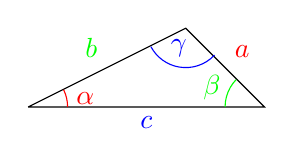
\begin{tikzpicture}
   \draw (0,0) -- (1.5,0) node[below,color=blue]{$c$} -- (3,0) --
   (2.5,.5)node[above right,color=red]{$a$} -- (2,1) --
   (1,.5)node[above left,color=green]{$b$} -- (0,0);

   \draw[color=red](.5,0) arc(0:13:.5) node[right]{$\alpha$}
   arc(13:26:.5);

   \draw[color=green](2.5,0) arc(180:150:.5) node[left]{$\beta$}
   arc(150:136:.5);

   \draw[color=blue](2.365676850809585,0.65900081996875) arc(-43:-100:.5)
   node[above]{$\gamma$} arc(-100:-152:.5);

 \end{tikzpicture}
\end{center}

\subsection{Ejercicio 1}

\begin{enumerate}
\item Exprese la ley de cosenos para $\cos \beta$ y $\cos \gamma$.
\item ¿Cómo interpretar el caso $\alpha = \frac{\pi}{2}$?
\item ¿Cómo interpretar el caso $\alpha = \pi$?
\item ¿Cómo interpretar el caso $\alpha = 0$?
\item Suponemos que $b = c$ y $\alpha = \frac{\pi}{3}$. Determine $a$.
\end{enumerate}

\subsection{Ejercicio 2 (recíproco del teorema de Pitágoras)}

Consideramos un triángulo con las notaciones precedientes.
Muestre que si $a^2 = b^2 + c^2$, el triángulo es rectángulo.

\subsection{Ejercicio 3}

Consideramos un triángulo con las notaciones precedientes. Determine una
aproximación de los lados y ángulos si

\begin{enumerate}
  \item Si $a=5\text{cm}$, $b=4\text{cm}$ y $c=7\text{cm}$ (caso L, L, L).
  \item Si $\alpha=55°$, $b=8\text{cm}$ y $c=5\text{cm}$ (caso L, A, L).
\end{enumerate}

\subsection{Ejercicio 4 (ley de cosenos)}

Consideramos las figuras siguientes donde $x$ es una distancia relativa.

\begin{center}
 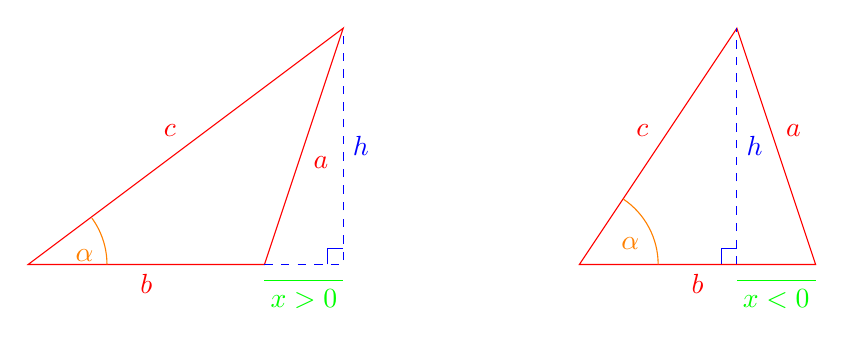
\begin{tikzpicture}
   \draw[color=red]
   (0,0) -- (1.5,0)node[below]{$b$} -- (3,0) --
   (3.5,1.5)node[below right]{$a$}  -- (4,3) -- 
   (2,1.5) node[above left]{$c$} -- cycle;
   \draw[color=blue,dashed](3,0)--(4,0)--(4,1.5)node[right]{$h$}--(4,3);
   \draw[color=blue](3.8,0)--(3.8,.2)--(4,.2);
   \draw[color=green](3,-.2) -- (3.5,-.2)node[below]{$x>0$} -- (4,-.2);
   \draw[color=orange](1,0) arc(0:18:1)node[below left]{$\alpha$} arc(18:36:1);
   
   \begin{scope}[shift={(7,0)}]
     \draw[color=red]
     (0,0) -- (1.5,0)node[below]{$b$} -- (3,0) --
     (2.5,1.5)node[above right]{$a$} --
     (2,3) -- (1,1.5)node[above left]{$c$} -- cycle;
     \draw[color=blue,dashed](2,0)--(2,1.5)node[right]{$h$}--(2,3);
     \draw[color=blue](1.8,0)--(1.8,.2)--(2,.2);
     \draw[color=green](3,-.2) -- (2.5,-.2)node[below]{$x<0$} -- (2,-.2);
     \draw[color=orange](1,0) arc(0:28:1)node[below left]{$\alpha$}
     arc(28:56:1);
   \end{scope}
 \end{tikzpicture}
\end{center}

\begin{enumerate}
\item Utilice el teorema de pítagoras en un triángulo rectángulo de hipotenusa
  $a$ para obtener una relación entre $a,h,x$.
\item Utilice el teorema de pítagoras en un triángulo rectángulo de hipotenusa
  $c$ para obtener una relación entre $h,b,x,c$.
\item Muestre $a^2 = c^2 - b^2 - {2bx}$.
\item Exprese $x$ en función de $c, b, \cos{\alpha}$.
\item Deduzca la ley de cosenos.
\end{enumerate}

\section{Ley de senos}

Sea un triángulo de ángulos $\alpha, \beta, \gamma$ con lados opuestos a estos
ángulos respectivamente $a,b,c$. Suponemos que
$0 < \alpha, \beta, \gamma < \pi$, es decir
$0 < \sin \alpha, \sin \beta, \sin \gamma \leq 1$. Tenemos las relaciones:

$$
\frac{a}{\sin \alpha} = \frac{b}{\sin \beta} =  \frac{c}{\sin \gamma}
$$

\subsection{Ejercicio 5 (triángulos isoceles)}

Consideramos un triángulo con las notaciones precedientes.

\begin{enumerate}
  \item Suponemos que $\alpha = \beta$. ¿Que decir de $a,b$?
  \item Suponemos que $a=b$. ¿Que decir de $\alpha, \beta$?
\end{enumerate}

\subsection{Ejercicio 6}

Consideramos un triángulo con las notaciones precedientes. Determine una
aproximación de los lados y ángulos si

\begin{enumerate}
  \item Si $b=\text{10cm}$, $\alpha = 20°$ y $\gamma = 55°$ (caso A, L, A)
  \item Si $a=\text{10cm}$, $b=\text{8cm}$ y $\alpha = 30°$.
  \item ¿Que decir del caso 
    $a=\text{8cm}$, $b=\text{10cm}$ y $\alpha=30°$?
\end{enumerate}

\subsection{Ejercicio 7 (ley de senos)}

Sea $ABC$ un triángulo consideramos su circunferencia circunscrita de centro
$O$ (se puede mostrar que siempre existe y por lo tanto $O$ es la interseción
de las mediatrices de los lados). Sea $D$ tal que $DC$ es un diámetro
y entonces $BCD$ rectángulo en $B$.

\begin{center}
 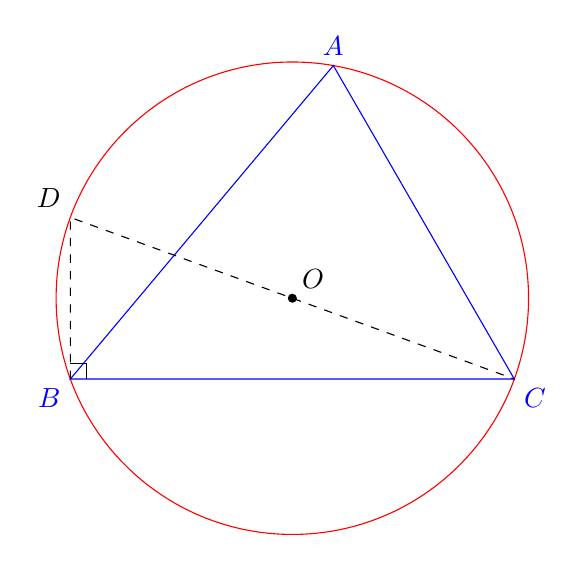
\begin{tikzpicture}
   \draw[color=red] (0,0) circle(3);
   \draw[color=blue]
   (0.52094453300079,2.954423259036624) node[above]{$A$} --
   (-2.819077862357725,-1.026060429977006) node[below left]{$B$} --
   (2.819077862357725,-1.026060429977006) node[below right]{$C$} -- cycle;
   \draw[fill=black] (0,0) node[above right]{$O$} circle(.05);

   \draw[dashed]
   (-2.819077862357725,-1.026060429977006) --
   (-2.819077862357725,1.026060429977006) node[above left]{$D$}--
   (2.819077862357725,-1.026060429977006);
   \draw 
   (-2.619077862357725,-1.026060429977006) --
   (-2.619077862357725,-.826060429977006) --
   (-2.819077862357725,-.826060429977006);
 \end{tikzpicture}
\end{center}

\begin{enumerate}
\item Exprese $\sin \widehat{D}$ en función de $a = BC$ y del radio
  $R = OA = OB = OC = OD$.
\item Utilice el teorema del ángulo inscrito
  (ejercicio 3 del capítulo V) para deducir 
  $\frac{a}{\sin \widehat{A}} = 2R$.
\item Deduzca la ley de senos. 
\end{enumerate}

\section{Soluciones de los ejercicios}

\subsection{Ejercicio 1}

\begin{enumerate}
\item 
  $$b^2 = c^2 + a^2 - {2ca \cos \beta}$$
  $$c^2 = a^2 + b^2 - {2ab \cos \gamma}$$

\item Si $\alpha = \frac{\pi}{2}$, $\cos \alpha = 0$ y el triángulo es
  rectángulo. Obtenemos el teorema de pítagoras: $a^2 = b^2+c^2$.
\item Si $\alpha = \pi$, $\cos \alpha = -1$ y el vértice corespondiente
  al ángulo $\alpha$ apartene al lado opuesto. Obtenemos 
  $a^2 = b^2 + c^2 + {2bc} = {b+c}^2$ es decir $a = b + c$.
\item Si $\alpha = 0$, $\cos \alpha = 1$ y los lados adyacentes al ángulo
  $\alpha$ son sobre la misma semirecta. Obentemos
  $a^2 = b^2 + c^2 - {2bc} = {b-c}^2$ es decir $a = b - c$ (si $b \geq c$) o
  $a = c - b$ (si $c \geq b$).  
\item Si $b = c$ y $\alpha = \frac{\pi}{3}$, obtenemos
  $a^2 = b^2 + b^2 - {2bc\frac{1}{2}} = b^2$ es decir $a=b=c$. En efecto
  eso coresponde a un triángulo equilatero.

\end{enumerate}

\subsection{Ejercicio 2 (recíproco del teorema de Pitágoras)}

$2bc \cos \alpha = a^2 - b^2 - c^2 = 0$. Porque $b, c > 0$ y
$0 \leq \alpha \leq \pi$, obtenemos $\alpha = \frac{\pi}{2}$ y el triángulo
es rectángulo.

\subsection{Ejercicio 3}

\begin{enumerate}
  \item 
    $\alpha =
    \arccos \left( \frac{a^2-b^2-c^2}{-2bc} \right) \approx 
    44°$,
    $\beta =
    \arccos \left( \frac{b^2-a^2-c^2}{-2ac} \right) \approx 34°$ y
    $\gamma =
    \arccos \left( \frac{c^2-a^2-b^2}{-2ab} \right) \approx 102°$.
  \item 
    $a = \sqrt{b^2 + c^2 - {2bc \cos \alpha}} \approx 
    6.57 \text{cm}$ entonces
    $\beta =
    \arccos \left( \frac{b^2-a^2-c^2}{-2ac} \right) \approx 86°$ y
    $\gamma =
    \arccos \left( \frac{c^2-a^2-b^2}{-2ab} \right) \approx 39°$.
\end{enumerate}

\subsection{Ejercicio 4 (ley de cosenos)}

\begin{enumerate}
\item $a^2 = h^2 + x^2$
\item $c^2 = h^2 + \left(b+x\right)^2$
\item Desde las relaciones precedientes, obtenemos
  $c^2 = h^2 + x^2 + {2bx} + b^2 = a^2 + {2bx} + b^2$ es decir
  $a^2 = c^2 - b^2 - {2bx}$.
\item $\cos \alpha = \frac{b+x}{c}$ entonces
  $x = {c \cos \alpha} - b$.
\item $a^2 = c^2 - b^2 - {2bx} = 
  c^2 - b^2 - {2b \left( {c \cos \alpha} - b \right)} =
  c^2 - b^2 - {bc\cos \alpha} + 2b^2$ y finalmente
  $$a^2 = b^2 + c^2 - {2bc \cos\alpha}$$
\end{enumerate}

\subsection{Ejercicio 5 (triángulos isoceles)}

\begin{enumerate}
  \item Si $\alpha=\beta$, $\sin \alpha = \sin \beta$ y
    entonces $a=b$.
  \item Si $a=b$, $\sin \alpha = \sin \beta$ es decir
    $\alpha = \beta$ o $\alpha = \pi - \beta$.
    Pero $\gamma = \pi - \alpha - \beta \neq 0$ y entonces $\alpha = \beta$.
\end{enumerate}

\subsection{Ejercicio 6}

\begin{enumerate}
\item $\beta = 180° - \alpha - \gamma = 105°$. Entonces
$a = \frac{b}{\sin \beta} \sin \alpha \approx
3.54 \text{cm}$ y
$c = \frac{b}{\sin \beta} \sin \gamma \approx 8.48 \text{cm}$

\item $\sin \beta = \frac{\sin \alpha}{a} \times b$
  entonces $\beta = \theta$ (y $\gamma = \pi - \alpha - \theta$) o
  $\beta = \pi - \theta$ (y $\gamma = \theta - \alpha$) donde
  $\theta = \arcsin \left(\frac{\sin \alpha}{a} \times b\right)$.
  Pero $\theta \approx 24° < 30° = \alpha$ entonces sólo el primer caso
  es posible: $\beta \approx 24°$, $\gamma \approx 126°$.
  Obtenemos 
    $c = \sqrt{a^2 + b^2 - {2ab \cos \gamma}} \approx 16.1\text{cm}$.

\item Ahora obtenemos $\theta \approx 39° > 30° = \alpha$ y entonces
  existen dos triángulos congruentes que satisfacen estas condiciones.
  
\end{enumerate}

\subsection{Ejercicio 7 (ley de senos)}

\begin{enumerate}
\item $\sin \widehat{D} = \frac{a}{2R}$.
\item Los ángulos inscritos $\widehat{A}, \widehat{D}$ 
  abarcan el mismo arco y entonces son iguales:
  $\frac{a}{\sin \widehat{A}} = \frac{a}{\sin \widehat{D}} = 2R$.
\item De la misma manera, podemos monstrar que
  $\frac{b}{\sin \widehat{B}} = 2R$ ($b = AC$) y
  $\frac{c}{\sin \widehat{C}} = 2R$ ($c = AB$). Finalmente
  %%
$$
\frac{a}{\sin \widehat{A}} = \frac{b}{\sin \widehat{B}} = 
\frac{c}{\sin \widehat{C}} = 2R
$$

\end{enumerate}

